
%(BEGIN_QUESTION)
% Copyright 2010, Tony R. Kuphaldt, released under the Creative Commons Attribution License (v 1.0)
% This means you may do almost anything with this work of mine, so long as you give me proper credit

A friend of yours has a table saw in his home workshop, which takes a long time to coast to a full stop after running.  He wants to put some kind of brake on the saw to bring the blade to a stop quicker, and he calls on you for help because you know some things about motors and motor controls.

Looking at the table saw, you see it is powered by a single-phase 240 VAC induction motor, through a DPDT on/off toggle switch with unused NC contacts:

$$\includegraphics[width=15.5cm]{i02431x01.eps}$$

\vskip 100pt

Modify the schematic diagram to include a pushbutton ``brake'' switch that electrically brakes the motor when pushed, and wire it in such a way that this braking feature cannot be engaged when the motor is powered by 240 VAC.  Your solution should be simple, not requiring the purchase of any expensive electronic devices (such as soft-starts or VFDs).

\underbar{file i02431}
%(END_QUESTION)





%(BEGIN_ANSWER)

This uses {\it DC injection braking} to slow down the motor:

$$\includegraphics[width=15.5cm]{i02431x02.eps}$$

Award only half credit for a workable solution that has no pushbutton (i.e. that immediately brakes when the power switch goes to the ``off'' position).

%(END_ANSWER)





%(BEGIN_NOTES)

{\bf This question is intended for exams only and not worksheets!}.

%(END_NOTES)

